\section{Results}
\subsection{Experiment 1a: Supervised classification test of scanner} \label{supervised_test}
After preprocessing, the images were converted to bias-field corrected, normalized, gray matter density maps, however site-related differences still existed in this dataset.

\begin{figure}[!ht]
\begin{center}
 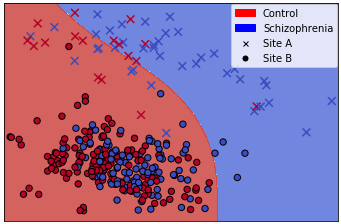
\includegraphics[width = 1\textwidth]{svm_decision_new_nobp.png}
    \end{center}
  \caption{The decision boundary, plotted in 2D, learned by a polynomial SVM when classifying diagnostic groups. The background colour represents the decision boundary. The colour of points represents the true diagnostic group membership, and the shape of points represents the scanners.}
  \label{fig:svm_decision}
\end{figure}

To illustrate the confounding influence that site-related differences can have on the ability to classify images, we initially performed a disease classification on our preprocessed (but untransformed) full dataset. Our full dataset contained images from two different groups and two different scanners. A polynomial SVM indicated the diagnostic groups were only weakly separable, and the decision boundary tended to separate scanners rather than clinical groups. Figure \ref{fig:svm_decision} shows a representation of the decision-boundary. The figure shows the decision-boundary (background colour) tends to separate shapes representing scanner differences (crosses and circles) rather than colours representing diagnostic differences (blue vs red). In particular, the crosses and circles are well-separated to the top right and bottom left of the figure, while the blue and red circles in the bottom left are intermingled. This impairs the accuracy of the model when using to predict unseen cases and favors the prediction of the sites rather than the clinical diagnosis.

We evaluated the ability of our generative adversarial network to remove the site-related differences in our dataset. We used the mid-sagittal slice from the T1-weighted MRI of healthy subjects from site A and site B, and we merged the distribution of each image set by transforming the images from site A into images that have similar morphological characteristics as site B.
Figure \ref{fig:transformation} shows a number of examples from the different sets and their resulting transformations. The transformed images (second row) demonstrate more consistency compared to the corresponding original images (top row). The differences between the original and transformed images, highlighted in the bottom row show significant changes in regions such as the thalamus and the brain stem.

Figure \ref{fig:mean_image} demonstrates the changes in the mean image before and after the transformation using the GAN. The top rightmost image in Figure \ref{fig:mean_image} shows that the differences in the mean of Site A and B are particularly localized to the thalamus and the frontal lobe, however after the transformation, the differences are not concentrated to a particular area of the brain. Similarly, the GAN brings the distribution of pixel intensities between Site A and B closer to each other as shown in Figure \ref{fig:pixel_distri}.

\begin{figure}[!ht]
\begin{center}
 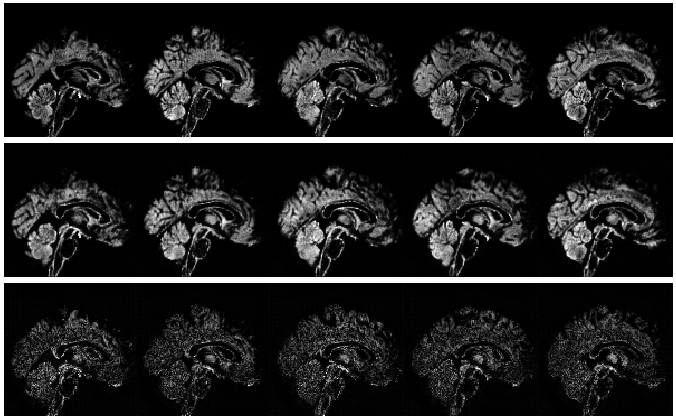
\includegraphics[width = 1\textwidth]{individual_differences.png}
    \end{center}
  \caption{\textbf{Top row}: Samples of images from site A. \textbf{Second row}: The result of the transformation of images from the top row using GAN. \textbf{Bottom row}: The absolute difference between the images of first and second row.}
  \label{fig:transformation}
\end{figure}

\begin{figure}[!ht]
\begin{center}
\begin{subfigure}[t]{0.43\linewidth}
\centering
 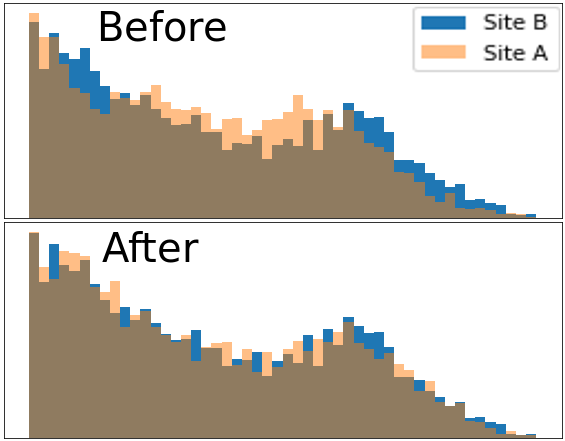
\includegraphics[width = 1\textwidth]{pixel_distribution_title.png}
 \caption{}
 \label{fig:pixel_distri}
 \end{subfigure}
 \hspace{0.1cm} % separation between the subfigures
\begin{subfigure}[t]{0.52\linewidth}

\centering
 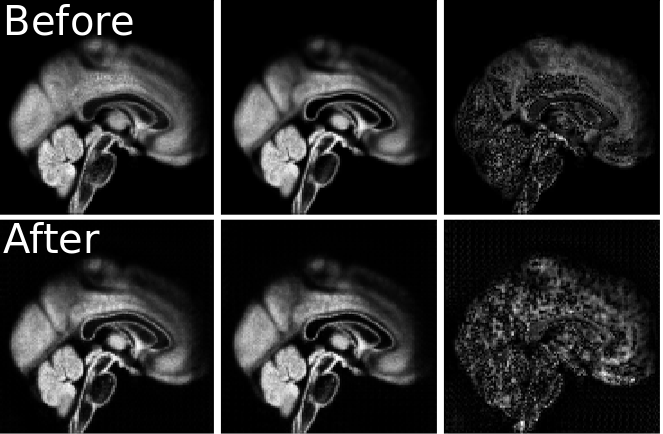
\includegraphics[width = 1\textwidth,height=1.6in]{mean_differences_title.png}
 \caption{}.

 \end{subfigure}
    \end{center}
  \caption{Change in the mean image distributions of Site A and B, before (top rows) and after (bottom rows) transformation to a common distribution. \textbf{(a)} Distribution of pixel intensity before and after transformation. \textbf{(b)} Mean image from Site A (left) and Site B (middle) and the mean difference (right), before and after transformation.}
  \label{fig:mean_image}
\end{figure}


We next conducted a supervised classification test of the dataset to determine how well the images from each site were distinguishable. A Gaussian SVM model was trained using the images from healthy controls. Table \ref{tab:classify_scanner} shows the performance of the classifier after different correctional techniques were applied to the healthy dataset, including linear regression, Gaussian regression, and our GAN transformation. The SVM was able to achieve close to 100 percent accuracy when discriminating between the two sites without any correction (99.3\% accuracy, 99.4\% precision, 99.3\% recall and 100\% specificity).  The linear correction method produced the worst outcome as the SVM was able to distinguish between the two site images with 100\% accuracy after application of this method. By contrast, the non-linear correction methods such as the GAN and GP regression reduced (but did not eliminate) the model's ability to distinguish between the sites. This suggests that the non-linear correction methods remove or minimise the site artifacts present in our dataset, with the GAN transformation producing the largest correction.

\begin{table}[!ht]
  \centering
  \caption{Classification of scanners, using different correctional methods. Average difference in performance from baseline (no correction) across 10-fold cross-validation. Bold indicates the best performing in the category. Standard deviation in square brackets.}
\begin{tabular}{l|cccc}
    \toprule
    \textbf{Correction method} & \textbf{Accuracy} & \textbf{Precision}& \textbf{Recall} & \textbf{Specificity}\\
    \midrule
    Linear regression   &  0.007 [0.0004] & 0.006 [0.0003] & 0.007 [0.0004] & 0.000 [0.0000]\\
    GP regression    &  -0.309 [0.0243] & \textbf{-0.476} [0.0353] & -0.309 [0.0243] & -0.049 [0.0036]\\
    GAN    & \textbf{-0.386} [0.0091] & -0.389 [0.0306]& \textbf{-0.386} [0.0091] & \textbf{-0.255}[0.0151] \\
    \bottomrule
    \end{tabular}%
  \label{tab:classify_scanner}%
\end{table}

\subsection{Experiment 1b: Unsupervised classification test of scanner} \label{unsupervised_test}

\begin{figure}[!ht]
\begin{center}
 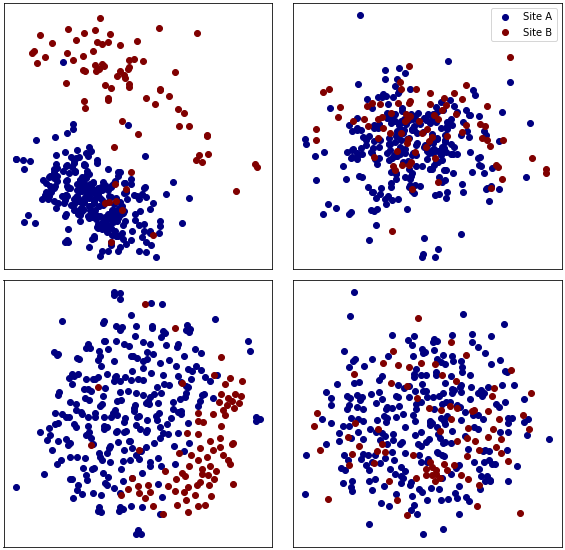
\includegraphics[width = 1\textwidth]{tsne_visualisation.png}
    \end{center}
  \caption{\textbf{Left column}: Images before transformation. \textbf{Right column}: Images after GAN transformation. \textbf{Top}: PCA visualisation of the two scanner sets. \textbf{Bottom}: a t-SNE visualisation}
  \label{fig:pca_tsne}
\end{figure}

We performed unsupervised learning to determine whether any unstructured information related to site differences remained in the dataset. Figure \ref{fig:pca_tsne} shows a 2D visualisation of the differences between data sets before and after the transformation by the GAN, using two dimensionality reduction techniques: principal component analysis (PCA) and t-Distributed Stochastic Neighbor Embedding (t-SNE) \citep{maaten2008visualizing}. t-SNE, unlike PCA, is a non-linear method that is useful for exploring local neighbourhoods and finding clusters in data. If data is naively pooled (left column), there is clear separation between the datasets from each site, suggesting that these site artifacts are a possible confound and will make any interpretation of results using pooled data difficult. However, after the GAN transformation (right column), such separation has vanished and the data is akin to that generated from the same distribution.

\subsection{Experiment 2: Classification of disease} \label{class_disease}
The previous experiment demonstrated the GAN transformation method removed site-related information from our dataset on the basis of supervised and unsupervised classification methods. An important concern is whether the information loss is selective to site differences or whether other information such as that related to clinical diagnosis, is also lost. To test that, we determined whether classification of clinical diagnosis was adversely affected by any of our correction methods. A Gaussian SVM was used to classify the diagnosis of the subjects as either healthy or schizophrenia. The SVM was able to achieve over 85 percent accuracy when discriminating between clinical diagnosis without any correction (87.1\% accuracy, 89.1\% precision, 87.1\% recall and 95.7\% specificity).   Table \ref{tab:classify_disease} shows comparisons compared to baseline using each correction method (Linear and GP regression, and GAN transformation).

\begin{table}[!ht]
  \centering
  \caption{Classification of disease, using different correctional methods. Average difference in performance from baseline (no correction) over each cross validation fold is reported. Bold indicates the best performing in the category. Negative values indicate a worse result compared to baseline. Standard deviation in square brackets.}
    \begin{tabular}{l|cccc}
    \toprule
    \textbf{Correction method} & \textbf{Accuracy} & \textbf{Precision}& \textbf{Recall} & \textbf{Specificity}\\
    \midrule
    Linear regression   &  -0.003 [0.0007] & 0.000 [0.0005]  & -0.003 [0.0007]  & \textbf{0.000} [0.0010]\\
    GP regression    &  0.025 [0.0010] & 0.021 [0.0010]  & 0.026 [0.0010] & -0.042 [0.0063]\\
    GAN    & \textbf{0.037} [0.0011] & \textbf{0.028} [0.0008]& \textbf{0.038} [0.0011]  & -0.043 [0.0032]\\
    \bottomrule
    \end{tabular}%
  \label{tab:classify_disease}%
\end{table}

Linear regression was the only method to produce negative changes in accuracy, implying it non-selectively removed information from our dataset. On the other hand, GP regression and GAN transformation produced significant improvements in accuracy, with GAN producing the largest improvement in accuracy (3.7\%) when compared to base and 1.2\% compared to GP regression. The negative changes in specificity after GP and GAN correction indicate there is some improvement of classification accuracy of the schizophrenia brain images at the expense of healthy brain images.

\subsection{Experiment 3: Classification of gender}
The GAN correction appears to selectively remove information related to site differences in our dataset, without adversely affecting information related to subtle clinical differences. However anatomical differences between psychiatric groups are likely to be small, obscure and perhaps not generally representative of the morphological changes produced by our correction methods here. Furthermore, the contribution of diagnostic groups from each site in our dataset is unbalanced (e.g., see Table \ref{tab:cohort}), and there are reasonable concerns that unbalanced sampling from confounded groups may artificially inflate classification accuracy, even after weighting for unbalanced groups \citep{rao2017predictive}. To help determine the general impact of our correction methods on anatomically distinct groups, and to eliminate concerns of inflated classification accuracy due to unbalanced groups, we tested the effect of GAN correction on balanced groups. We created a dataset which balanced the group contribution from each site by randomly selecting a set of 37 male images and 37 female images from each site. Thus, we balanced both gender and site in this dataset. Male and female images from each site were then pooled together, and correction methods were applied to each dataset. We then tested whether a Gaussian SVM could classify brain images by gender. On a balanced dataset, the baseline classification accuracy of the SVM (i.e., uncorrected images) was less than 70 percent (65.2\% accuracy, 65.6\% precision, 64.5\% recall and 65.9\% specificity). The results of our correction methods are shown in Table \ref{tab:classify_gender}. The GAN corrected images improved accuracy by 15.8\% compared to baseline whereas linear regression and GP regression produced no significant difference in the classification of gender from baseline (and on average they even reduced classification performance).

\begin{table}[ht!]
  \centering
  \caption{Classification of gender, using different correctional methods. Reported values correspond to the average of the differences of each cross validation fold test between baseline (no correction) and the correction method. Bold indicates the best performing in the category. Negative values indicate a worse result compared to baseline. Standard deviation in square brackets.}
    \begin{tabular}{l|ccccc}
    \toprule
    \textbf{Correction method} & \textbf{Accuracy} & \textbf{Precision}& \textbf{Recall}& \textbf{Specificity}\\
    \midrule
    Linear regression   &  -0.015 [0.0027] & -0.018 [0.0032] & -0.016 [0.0053] & -0.014 [0.0018]\\
    GP regression    &  -0.033 [0.0026] & -0.036 [0.0022] & -0.025 [0.0056] & -0.041 [0.0071]\\
    GAN    & \textbf{0.158} [0.0332] & \textbf{0.130} [0.0362] & \textbf{0.211} [0.0310] & \textbf{0.105}[0.0576]\\
    \bottomrule
    \end{tabular}%
  \label{tab:classify_gender}%
\end{table}

\subsection{Experiment 4: Reconstruction}

\begin{figure}[!ht]
\begin{center}
 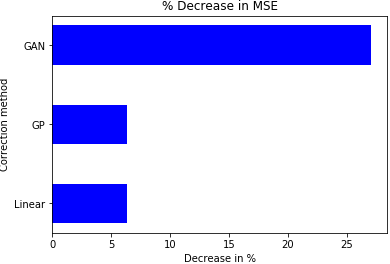
\includegraphics[width = 1\textwidth]{mse.png}
    \end{center}
  \caption{Percentage decrease in reconstruction (MSE) error against baseline for the different correction methods.}
  \label{fig:mse}
\end{figure}

11 subjects (5 male) had undergone MRI scans at site A and site B. This allowed us to determine how similar the reconstructed images from the different methods were to images of the same brain collected at the actual site. Images from site B were corrected to site A and were compared to the actual images collected at site A for the selected subjects. The mean square error (MSE) between the corrected and actual image for each subject was calculated and was compared to baseline. Linear regression and GP regression performed similar to each other with a 6.35\% decrease in error. The GAN correction had significant improvement over the other regression methods with a 27.02\% decrease in error.

\begin{comment}
\begin{table}[ht!]
  \centering
  \caption{The percentage change from baseline in mean square error of the transformed images of site A and original site B for 11 subjects using different correction methods. A negative result indicates a worse performance compared to baseline.}
	\begin{tabular}{l|c}
    \toprule
    \textbf{Correction method} & \textbf{Change in MSE \%} \\
    \midrule
    Linear regression   &  6.34 \\
    GP regression    &  6.35 \\
    GAN    & \textbf{18.74} \\
    \bottomrule
    \end{tabular}%
  \label{tab:reconstruction}%
\end{table}
\end{comment}
